\documentclass[9pt, aspectratio=169]{beamer}
%\documentclass[9pt, handout, aspectratio=169]{beamer} % makes just 1 slide for each frame (handout)

% language support
\usepackage[english]{babel}

% packages for figures
\usepackage{graphicx}
\usepackage{subcaption}

% math and physics packages
\usepackage{amssymb}
\usepackage{amsmath}
\usepackage{physics}
\usepackage{bm}
%\usepackage[compat=1.1.0]{tikz-feynman} % to create feynman diagrams
\DeclareMathOperator{\sign}{Sign}
\usepackage{tikz}
\usetikzlibrary{arrows, automata, positioning, shapes.geometric}
\definecolor{color1}{RGB}{5, 213, 250}
\definecolor{color2}{RGB}{0,0,139}
\definecolor{color3}{RGB}{227,26,28}
\definecolor{color4}{RGB}{127,255,0}
\definecolor{color5}{RGB}{255,255,0}
\definecolor{color6}{RGB}{139,69,19}
\definecolor{color7}{RGB}{255,127,0}
\definecolor{color8}{RGB}{106,61,154}
\definecolor{color9}{RGB}{255,105,180}
\definecolor{color10}{RGB}{109,113,46}
\usepackage[style=verbose,backend=biber,doi=false,isbn=false,url=false]{biblatex}
\addbibresource{references.bib}
\setbeamertemplate{bibliography item}{}

\setbeamercolor{postit}{fg=black,bg=white!80!green}


% other packages
\usepackage{multicol}
\usepackage{verbatim} % for the \begin{comment} command


% settings for theme/font
%%%%%%%%%%%%%%%%%%%%%%%%%
\usepackage{appendixnumberbeamer} % no page number in appendix
\usetheme[progressbar=frametitle]{metropolis}
\setbeamercolor{background canvas}{bg=white}
% \usefonttheme[onlymath]{serif} % use "standard" font for math symbols
\setbeamertemplate{frametitle continuation}[from second][] % prevents numbering of content frame if it contains a frame break

\addtobeamertemplate{footline}{% add navigation bar and frame number at bottom
    \leavevmode
    \hbox{
    \begin{beamercolorbox}[wd=0.88\paperwidth,ht=2.75ex,dp=3.0ex,left,leftskip=1em]{}
        \usebeamercolor[fg]{navigation symbols}{\insertslidenavigationsymbol \insertframenavigationsymbol \insertsectionnavigationsymbol}
    \end{beamercolorbox}
    \begin{beamercolorbox}[wd=0.1\paperwidth,ht=2.5ex,dp=3.0ex,right,rightskip=1em]{footlinenum}
        \insertframenumber{} / \inserttotalframenumber
        \vskip 0.07pt
    \end{beamercolorbox}
    }
}{}


% Definitions of handy macros
%%%%%%%%%%%%%%%%%%%%%%%%%%%%%
\newcommand{\m}[1]{\mathrm{#1}}
\newcommand{\todo}[2][\huge]{\textcolor{red}{\fbox{#1#2}}} % to add red todo boxes
\newcommand<>{\uncoverubrace}[2]{% to cover/uncover underbraces
    \onslide#3 \underbrace{ \onslide<1->%
    #1%
    \onslide#3 }_{#2} \onslide<1->%
}

\let\phi\varphi
\let\epsilon\varepsilon

% to insert a tab
\newcommand{\tab}[0]{\phantom{1234}}




\title{Cluster Algorithm for the 1+1 Dimensional $S=1/2$ Quantum Link Model}
%\subtitle{}
\author{Thea Budde}
\institute{ETH Zürich \\
Supervisors: Joao C. Pinto Barros, Marina Krstic Marinkovic}
\date{21.03.23}

\begin{document}
\metroset{block=fill}

\begin{frame}
	\titlepage
\end{frame}


\begin{frame}[t]{Motivation}
    \begin{itemize}
        \setlength{\itemsep}{0.3cm}
        \item Lattice QCD is very successful, but many unsolved problems remain
        \item The search for alternative techniques is ongoing
        \pause
        \item Quantum simulators are a promising future technology, but still limited
        \pause
        \item Quantum link models have already been implemented\footcite{Surace2019, Zhou2021}
        \pause
        \item Classical algorithms benchmark quantum simulators and probe quantum supremacy
        \pause
        \item Solving toy models can give insight to solving more complicated systems
    \end{itemize}
\end{frame}


% frame with table of contents (which allows frame breaks)
\begin{frame}[allowframebreaks, t]
	\frametitle{Content}
	\setbeamertemplate{section in toc}[sections numbered]
    \tableofcontents
\end{frame}

\section{$S = 1/2$ Quantum Link Model}

\begin{frame}[t]{$S = 1/2$ Quantum Link Model}
    \begin{itemize}
        \setlength{\itemsep}{0.3cm}

        \item Similar to the Schwinger model, so 1+1 dimensional QED
        \item A short derivation in the Hamlitonian formalism:
        \pause
        \begin{itemize}
            \setlength{\itemsep}{0.1cm}
            \item Start with continuous Dirac Hamiltonian in 1+1 dimensions
            \begin{equation*}
                H = \int d x \bar{\psi} (i \partial_\mu \gamma^\mu - m)\psi
            \end{equation*}
            \pause
            \item Discretize space and derivative to a finite volume $L = N a$
            \pause
            \item A spinor is represented by two lattice sites
            \begin{equation*}
                \psi_n = \frac{1}{\sqrt{a_{st}}} 
                \begin{pmatrix}
                    c_{2n} \\
                    c_{2n+1}
                \end{pmatrix}
            \end{equation*}
            \pause
        \end{itemize}

    \vspace{-0.2cm}


    \begin{figure}[t]
        \centering
        \resizebox{0.4\textwidth}{!}{
        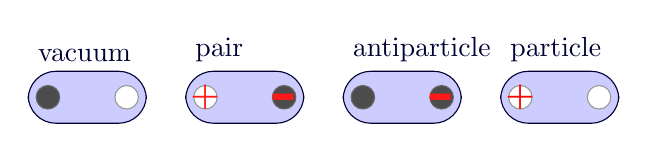
\begin{tikzpicture}[xscale = 1, yscale = 0.66]

            \draw[blue!20!black,fill=blue!20,rounded corners=10]
                (-0.25,0.5) node[above right] {vacuum} rectangle (1.25,-0.5);

            \draw[blue!20!black,fill=blue!20,rounded corners=10]
                (1.75, 0.5) node[above right] {pair} rectangle (3.25,- 0.5);

            \draw[blue!20!black,fill=blue!20,rounded corners=10]
                (3.75,0.5) node[above right] {antiparticle} rectangle (5.25,-0.5);

            \draw[blue!20!black,fill=blue!20,rounded corners=10]
                (5.75, 0.5) node[above right] {particle} rectangle (7.25,-0.5);
            
            \foreach \x in {0,3,4,5}
            \node [draw, circle, fill=white!30!black, minimum size=.1cm, scale=0.9, draw=white!40!black] at (\x,0) {};
        
            \foreach \x in {1,2,6,7}
            \node [draw, circle, fill=white, minimum size=.1cm, scale=0.9, draw=white!60!black] at (\x,0) {};
        
            \node[align=left, text=white!10!red,font=\large] at (1.998,0) {\textbf{+}};
            \node[align=left, text=white!10!red,font=\Huge] at (3.016,0) {\textbf{-}};
            \node[align=left, text=white!10!red,font=\Huge] at (5.016,0) {\textbf{-}};
            \node[align=left, text=red,font=\large] at (5.998,0) {\textbf{+}};
        \end{tikzpicture}}
        
    \end{figure}
\end{itemize}

\end{frame}

\begin{frame}[t]{$S = 1/2$ Quantum Link Model}
    \begin{itemize}
        \setlength{\itemsep}{0.3cm}
        \item The Hamiltonian becomes
        \begin{equation*}
            H = \sum_{n=0}^{N-1} \left( - \frac{i}{2a} c_n^{\dagger}c_{n+1} + h.c. + m (-1)^n c_n^{\dagger} c_n \right)
        \end{equation*}
        \vspace{-0.4cm}
        \pause
        \item Now we introduce the gauge field
        \item We want $U(1)$ symmetry under the transformation $c_n \to e^{i\alpha_n} c_n$
        \item Introduce link variables such that $c_n^\dagger  U_{n,n+1} c_{n+1}$ is invariant
        \begin{align*}
            U_{n,n+1} \to e^{i\alpha_n}  U_{n,n+1} e^{-i\alpha_{n+1}} && [U_n, E_m] = e \delta_{nm} U_n^\dagger
        \end{align*}
        \pause
        \vspace{-0.8cm}
        \item A gauge invariant Hamiltonian is given by
        \begin{equation*}
            H = \frac{i}{2a} \sum_n (c_n^\dagger U_n c_{n+1}  - c_{n+1}^\dagger U_n^\dagger c_n ) + m \sum_n (-1)^n c_n^\dagger c_n + \frac{a}{2} \sum_n E_n^2
        \end{equation*}
    \end{itemize}
\end{frame}

\begin{frame}[t]{$S = 1/2$ Quantum Link Model}
    \begin{itemize}
        \setlength{\itemsep}{0.2cm}
        \item Gauge symmetry manifests in generators $G_n$ that commute with the Hamiltonian
        \begin{equation*}\label{eq:gauss_law}
            G_n = \frac{1}{e} E_{n} - \frac{1}{e}  E_{n-1} - c_n^\dagger c_n + \frac{1 - (-1)^n}{2}.
        \end{equation*}
        \item Gauss's Law: Only states with $G_n \ket{\psi} = 0$ are physical
        \pause
        \item Gauss's law ensures that the difference between the left and right link of
        \begin{itemize}
            \setlength{\itemsep}{0.1cm}
            \item a positively charged particle, so an even flipped site is 1
            \item a negatively charged particle, so an odd flipped site is -1
            \item the vacuum, so an unflipped site is 0
        \end{itemize}
    \end{itemize}

    \vspace{0.4cm}

    \begin{figure}[t]
        \centering
        \resizebox{0.5\textwidth}{!}{
        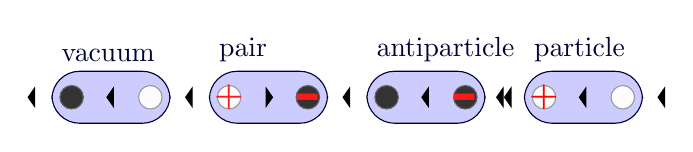
\begin{tikzpicture}[xscale = 1, yscale = 0.66]

            \draw[blue!20!black,fill=blue!20,rounded corners=10]
                (-0.25,0.5) node[above right] {vacuum} rectangle (1.25,-0.5);

            \draw[blue!20!black,fill=blue!20,rounded corners=10]
                (1.75, 0.5) node[above right] {pair} rectangle (3.25,- 0.5);

            \draw[blue!20!black,fill=blue!20,rounded corners=10]
                (3.75,0.5) node[above right] {antiparticle} rectangle (5.25,-0.5);

            \draw[blue!20!black,fill=blue!20,rounded corners=10]
                (5.75, 0.5) node[above right] {particle} rectangle (7.25,-0.5);

            \foreach \x in {0,3,4,5}
            \node [draw, circle, fill=white!20!black, minimum size=.1cm, scale=0.9, draw=white!40!black] at (\x,0) {};
        
            \foreach \x in {1,2,6,7}
            \node [draw, circle, fill=white!99!black, minimum size=.1cm, scale=0.9, draw=white!60!black] at (\x,0) {};

            \node[align=left, text=white!10!red,font=\large] at (1.998,0) {\textbf{+}};
            \node[align=left, text=white!10!red,font=\Huge] at (3.016,0) {\textbf{-}};
            \node[align=left, text=white!10!red,font=\Huge] at (5.016,0) {\textbf{-}};
            \node[align=left, text=red,font=\large] at (5.998,0) {\textbf{+}};

            \foreach \x in {0,1,2,4,5,7,8}
            \node[isosceles triangle, isosceles triangle apex angle=110,
                draw,fill=black, minimum size =0.03cm, inner sep=0.03cm, rotate=180] (T60) at (-0.5 + \x, 0){};

            \node[isosceles triangle, isosceles triangle apex angle=110,
                draw,fill=black, minimum size =0.03cm, inner sep=0.03cm] (T60) at (2.5, 0){};

            \node[isosceles triangle, isosceles triangle apex angle=110,
                draw,fill=black, minimum size =0.03cm, inner sep=0.03cm, rotate=180] (T60) at (5.45, 0){};
            \node[isosceles triangle, isosceles triangle apex angle=110,
                draw,fill=black, minimum size =0.03cm, inner sep=0.03cm, rotate=180] (T60) at (5.55, 0){};
        \end{tikzpicture}}
    \end{figure}
\end{frame}

\begin{frame}[t]{$S = 1/2$ Quantum Link Model}
    \begin{itemize}
        \setlength{\itemsep}{0.3cm}
        \item This (Wilson formulation) still approaches the Schwinger model in the small lattice spacing limit
        \pause
        \item Now a restriction to a finite Hilbert space is introduced
        \item The field may only take spin values 
        \begin{align*}
            E_n = e \, S_n^z && U_n \to L_{+n} = \frac{1}{\sqrt{S(S+1)}} (S_n^x + i S_n^y)
        \end{align*}
        \vspace{-0.4cm}
        \pause
        \item Still a gauge symmetric theory, but $U_n$ is no longer unitary
        %\item In the limit $S \to  \infty$ the Wilson formulation is restored
    \end{itemize}
    \pause
    
    \begin{figure}[t]
        \centering
        \resizebox{0.5\textwidth}{!}{
        \only<4>{
            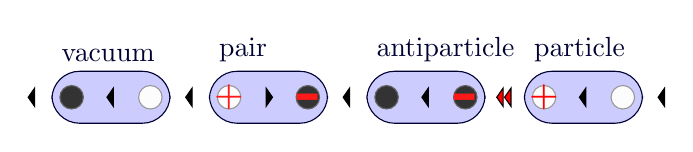
\begin{tikzpicture}[xscale = 1, yscale = 0.66]

            \draw[blue!20!black,fill=blue!20,rounded corners=10]
                (-0.25,0.5) node[above right] {vacuum} rectangle (1.25,-0.5);

            \draw[blue!20!black,fill=blue!20,rounded corners=10]
                (1.75, 0.5) node[above right] {pair} rectangle (3.25,- 0.5);

            \draw[blue!20!black,fill=blue!20,rounded corners=10]
                (3.75,0.5) node[above right] {antiparticle} rectangle (5.25,-0.5);

            \draw[blue!20!black,fill=blue!20,rounded corners=10]
                (5.75, 0.5) node[above right] {particle} rectangle (7.25,-0.5);
            
            \foreach \x in {0,3,4,5}
            \node [draw, circle, fill=white!20!black, minimum size=.1cm, scale=0.9, draw=white!40!black] at (\x,0) {};
        
            \foreach \x in {1,2,6,7}
            \node [draw, circle, fill=white!99!black, minimum size=.1cm, scale=0.9, draw=white!60!black] at (\x,0) {};
            
            \foreach \x in {0,1,2,4,5,7,8}
            \node[isosceles triangle, isosceles triangle apex angle=110,
                draw,fill=black, minimum size =0.03cm, inner sep=0.03cm, rotate=180] (T60) at (-0.5 + \x, 0){};

            \node[isosceles triangle, isosceles triangle apex angle=110,
                draw,fill=black, minimum size =0.03cm, inner sep=0.03cm] (T60) at (2.5, 0){};

            \node[isosceles triangle, isosceles triangle apex angle=110,
                draw,fill=red, minimum size =0.03cm, inner sep=0.03cm, rotate=180] (T60) at (5.45, 0){};
            \node[isosceles triangle, isosceles triangle apex angle=110,
                draw,fill=red, minimum size =0.03cm, inner sep=0.03cm, rotate=180] (T60) at (5.55, 0){};
                \node[align=left, text=white!10!red,font=\large] at (1.998,0) {\textbf{+}};
                \node[align=left, text=white!10!red,font=\Huge] at (3.016,0) {\textbf{-}};
                \node[align=left, text=white!10!red,font=\Huge] at (5.016,0) {\textbf{-}};
                \node[align=left, text=red,font=\large] at (5.998,0) {\textbf{+}};
            \end{tikzpicture}}%
        \only<5,6>{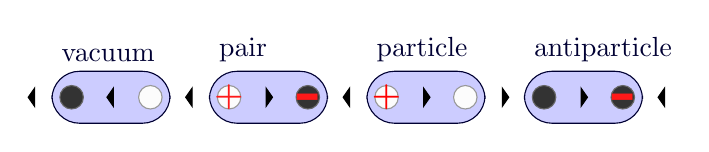
\begin{tikzpicture}[xscale = 1, yscale = 0.66]

            \draw[blue!20!black,fill=blue!20,rounded corners=10]
                (-0.25,0.5) node[above right] {vacuum} rectangle (1.25,-0.5);

            \draw[blue!20!black,fill=blue!20,rounded corners=10]
                (1.75, 0.5) node[above right] {pair} rectangle (3.25,- 0.5);

            \draw[blue!20!black,fill=blue!20,rounded corners=10]
                (3.75,0.5) node[above right] {particle} rectangle (5.25,-0.5);

            \draw[blue!20!black,fill=blue!20,rounded corners=10]
                (5.75, 0.5) node[above right] {antiparticle} rectangle (7.25,-0.5);
            
            \foreach \x in {0,3,6,7}
            \node [draw, circle, fill=white!20!black, minimum size=.1cm, scale=0.9, draw=white!40!black] at (\x,0) {};
        
            \foreach \x in {1,2,4,5}
            \node [draw, circle, fill=white!99!black, minimum size=.1cm, scale=0.9, draw=white!60!black] at (\x,0) {};
            
            \foreach \x in {0,1,2,4,8}
            \node[isosceles triangle, isosceles triangle apex angle=110,
                draw,fill=black, minimum size =0.03cm, inner sep=0.03cm, rotate=180] (T60) at (-0.5 + \x, 0){};
            
            \foreach \x in {3,5,6,7}
            \node[isosceles triangle, isosceles triangle apex angle=110,
                draw,fill=black, minimum size =0.03cm, inner sep=0.03cm] (T60) at (-0.5 + \x, 0){};
            \node[align=left, text=white!10!red,font=\large] at (1.998,0) {\textbf{+}};
            \node[align=left, text=white!10!red,font=\Huge] at (3.016,0) {\textbf{-}};
            \node[align=left, text=white!10!red,font=\Huge] at (7.016,0) {\textbf{-}};
            \node[align=left, text=red,font=\large] at (3.998,0) {\textbf{+}};
            \end{tikzpicture}}
        }
    \end{figure}%
    \only<6>{
    \begin{itemize}
        \item For the $S = 1/2$ model positive and negative sites need to alternate
    \end{itemize}
    }
\end{frame}

\begin{frame}[t]{Summary}
    \begin{itemize}
        \setlength{\itemsep}{0.3cm}
        \item We want to simulate the Hamiltonian
        \begin{equation*}
            H = \frac{i}{2a} \sum_n (c_n^\dagger U_n c_{n+1}  - c_{n+1}^\dagger U_n^\dagger c_n ) + m \sum_n (-1)^n c_n^\dagger c_n + \frac{a}{2} \sum_n E_n^2
        \end{equation*}
        \item[] on the Hilbert space that obeys Gauss's law and where the field only takes values $\{-1/2, 1/2\}$
        \pause
        \item These configurations are the chains of fermions where even and odd sites are flipped alternatingly relative to the vacuum.
    \end{itemize}
    \begin{figure}
    \centering
    \resizebox{0.5\textwidth}{!}{
    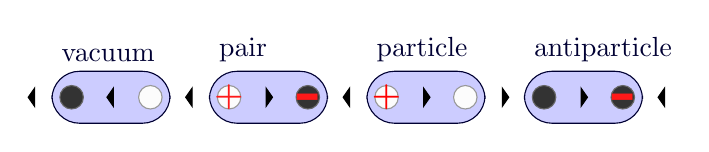
\begin{tikzpicture}[xscale = 1, yscale = 0.66]

        \draw[blue!20!black,fill=blue!20,rounded corners=10]
            (-0.25,0.5) node[above right] {vacuum} rectangle (1.25,-0.5);

        \draw[blue!20!black,fill=blue!20,rounded corners=10]
            (1.75, 0.5) node[above right] {pair} rectangle (3.25,- 0.5);

        \draw[blue!20!black,fill=blue!20,rounded corners=10]
            (3.75,0.5) node[above right] {particle} rectangle (5.25,-0.5);

        \draw[blue!20!black,fill=blue!20,rounded corners=10]
            (5.75, 0.5) node[above right] {antiparticle} rectangle (7.25,-0.5);
        
        \foreach \x in {0,3,6,7}
        \node [draw, circle, fill=white!20!black, minimum size=.1cm, scale=0.9, draw=white!40!black] at (\x,0) {};
    
        \foreach \x in {1,2,4,5}
        \node [draw, circle, fill=white!99!black, minimum size=.1cm, scale=0.9, draw=white!60!black] at (\x,0) {};
        
        \foreach \x in {0,1,2,4,8}
        \node[isosceles triangle, isosceles triangle apex angle=110,
            draw,fill=black, minimum size =0.03cm, inner sep=0.03cm, rotate=180] (T60) at (-0.5 + \x, 0){};
        
        \foreach \x in {3,5,6,7}
        \node[isosceles triangle, isosceles triangle apex angle=110,
            draw,fill=black, minimum size =0.03cm, inner sep=0.03cm] (T60) at (-0.5 + \x, 0){};
        \node[align=left, text=white!10!red,font=\large] at (1.998,0) {\textbf{+}};
        \node[align=left, text=white!10!red,font=\Huge] at (3.016,0) {\textbf{-}};
        \node[align=left, text=white!10!red,font=\Huge] at (7.016,0) {\textbf{-}};
        \node[align=left, text=red,font=\large] at (3.998,0) {\textbf{+}};
        \end{tikzpicture}}
    \end{figure}%
\end{frame}

\section{Meron Cluster Algorithm}

\begin{frame}[t]{Meron Cluster Algorithm}
    \begin{itemize}
        \setlength{\itemsep}{0.3cm}
        \item Foundation given by algorithm introduced by Chandrasekharan and Wiese\footcite{Chandrasekharan1999, Chandrasekharan2003}
        \item Algorithm to simulate spinless fermions with a nearest neighbor interaction
        \begin{equation*}
            H = \sum_{n=0}^{N}  -t (c_n^\dagger c_{n+1} + c_{n+1}^\dagger c_n) +  m \sum_n (-1)^n c_n^\dagger c_n  + U \left(c_n^\dagger c_n - \frac{1}{2}\right) \left(c_{n+1}^\dagger c_{n+1} - \frac{1}{2}\right)
        \end{equation*}
        \item No gauge field
        \item Constraint $U = 2t$ and $m = 0$ needed for this approach
    \end{itemize}
\end{frame}

\begin{frame}[t]{Meron Cluster Algorithm}
    \begin{itemize}
        \item We want to calculate observables via the partition function
        \begin{equation*}
            Z = \Tr \left\{ \exp [-\beta H] \right\}
        \end{equation*}
        \item Trotterize
        \begin{align*}
            H_{\text{even}} = \sum_{n=0}^{N/2} h_{2n} && H_{\text{odd}} = \sum_{n=0}^{N/2} h_{2n + 1}
        \end{align*}
        \begin{equation*}
            Z = \Tr \left\{ \exp [-\beta H] \right\} = \Tr \left\{ \exp [-\frac{\beta}{M} H_{\text{even}}] \exp [-\frac{\beta}{M} H_{\text{odd}}] \right\}^M + \mathcal{O}\left(\frac{\beta}{M}\right),
        \end{equation*}
        \pause
        \vspace{-0.4cm}
        \item Insert complete sets of fermion Fock basis states (with $\epsilon = \beta/M$)
        \begin{align*}
            Z = \sum_{n_0,n_1,n_2,n_3,...} \bra{n_0} \exp [-\epsilon H_{\text{even}}] \ket{n_1} \bra{n_1} \exp [-\epsilon H_{\text{odd}}] \ket{n_2} \bra{n_2} ... \ket{n_0}
        \end{align*} 
    \end{itemize}
\end{frame}


\begin{frame}[t]{Meron Cluster Algorithm}
    \begin{itemize}
        \item These terms can be represented on a 1+1 dimensional lattice
    \begin{equation*}
        Z = \sum_{n_0,n_1,n_2,n_3,...} \bra{n_0} \exp [-\epsilon H_{\text{even}}] \ket{n_1} \bra{n_1} \exp [-\epsilon H_{\text{odd}}] \ket{n_2} \bra{n_2} ... \ket{n_0}
    \end{equation*}
    \end{itemize}
    \vspace{-0.3cm}
    \only<1>{
        \begin{figure}
            \includegraphics[width=0.6\textwidth]{Figures/plaquette_no_weights.pdf}
        \end{figure}
    }
    \only<2>{
    \begin{figure}
        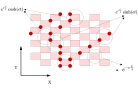
\includegraphics[width=0.6\textwidth]{Figures/plaquette_weights.pdf}
    \end{figure}
    \vspace{-0.6cm}
    \begin{itemize}
        \item Weight of configuration is the product of plaquette weights
    \end{itemize}
    }
\end{frame}

\begin{frame}[t]{Meron Cluster Algorithm}
    \begin{columns}[t]
    \column{0.6\textwidth}
        \begin{itemize}
            \setlength{\itemsep}{0.6cm}
            \item Split weights over break-ups $b$
            \begin{equation*}
                 \bra{n_i} \exp [-\epsilon h] \ket{n_{i+1}} = \exp(-s[n]) = \sum_b \exp(-s[n,b]) 
            \end{equation*}
            \only<2,3>{
            \item Sample over fermion and break-up configurations
            \begin{equation*}
                Z = \sum_{[n]} \exp(-S[n]) \to Z = \sum_{[n,b]} \exp(-S[n,b])
            \end{equation*}}
            \only<3>{
            \item Calculate observables as
            \begin{equation*}
                \langle O \rangle_f = \frac{1}{Z} \sum_{[n,b]} O[n] \exp(-S[n,b])
            \end{equation*}}
        \end{itemize}
    \column{0.4\textwidth}
        \begin{figure}
            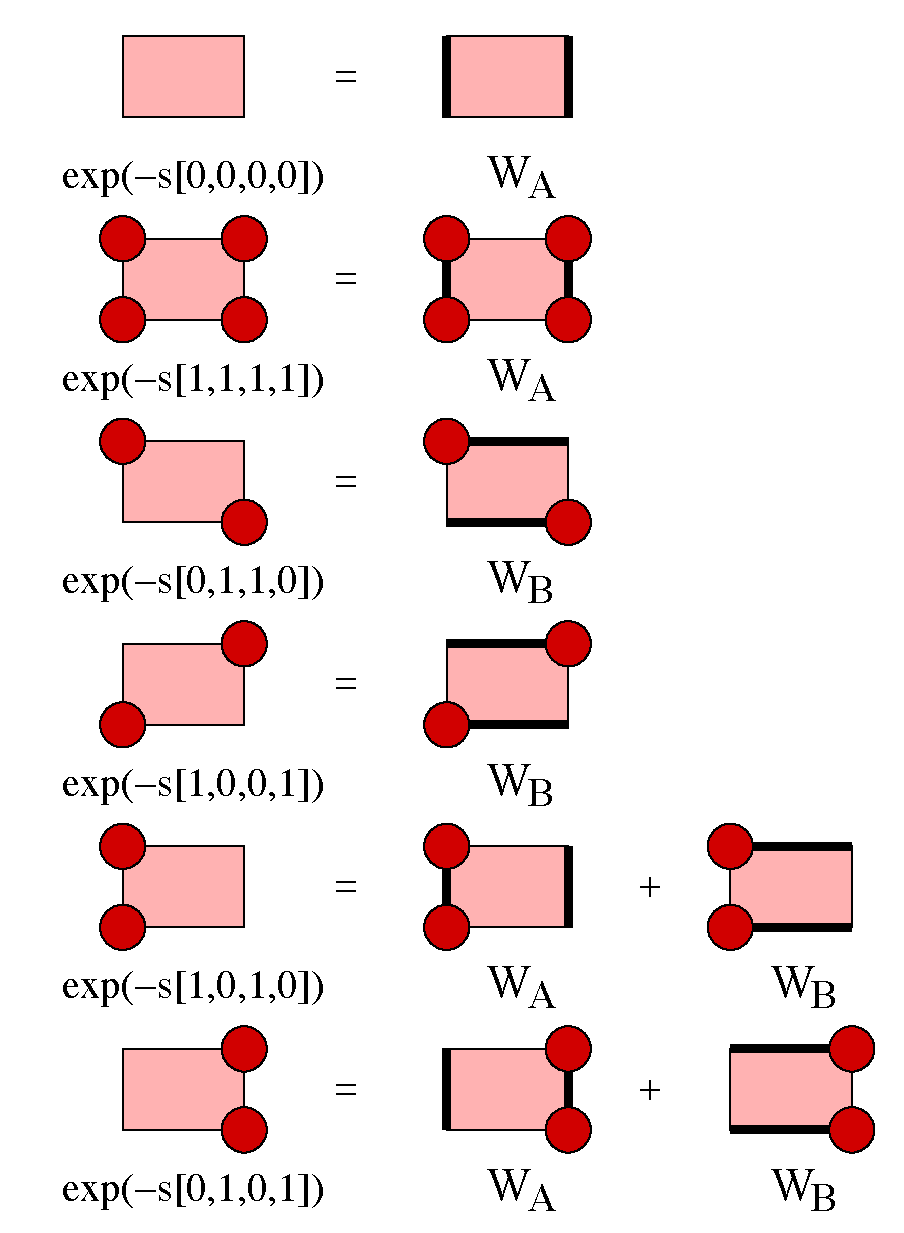
\includegraphics[width=0.8\textwidth]{Figures/bond_equation.pdf}
        \end{figure}
    \end{columns}
\end{frame}

\begin{frame}[t]{Meron Cluster Algorithm}
    \begin{itemize}
        \item The break-ups form loops on the periodic lattice, called clusters
        \begin{figure}
            \includegraphics[trim={3cm 19cm 3cm 3cm},width=0.9\textwidth]{Figures/bond_example.pdf}
        \end{figure}
        \item All configurations reachable with flips are in the Hilbert space
    \end{itemize}
\end{frame}

\begin{frame}[t]{Meron Cluster Algorithm}
    \begin{itemize}
        \setlength{\itemsep}{0.5cm}
        \item Summary of the steps of the meron cluster algorithm:
        \begin{enumerate}
            \setlength{\itemsep}{0.3cm}
            \item Place break-ups
            \item Flip each cluster with $p_{\text{flip}} = 0.5$
        \end{enumerate}
        \item This is ergotic and satisfies detailed balance
        \item However, Gauss's law is not satisfied!
    \end{itemize}
\end{frame}

\section{$S = 1/2$ Cluster Algorithm}

\begin{frame}[t]{$S = 1/2$ Cluster Algorithm}
    \begin{itemize}
        \setlength{\itemsep}{0.4cm}
        \item This brings us to the question of my thesis:
        \begin{center}
            \hspace{1cm}
            \begin{beamercolorbox}[sep=0.8em,wd=12.4cm]{postit}
                How can we ensure that the algorithm is restricted to physical $S=1/2$ configurations?
            \end{beamercolorbox}
        \end{center}
        \pause
        \item Generating a random flip out of the $2^n$ options and accepting the new configuration only if it is physical, scales exponentially with the volume
        \pause
        \item I constructed an algorithm that generates a random physical configuration in $\mathcal{O}(V)$ steps
    \end{itemize}
\end{frame}

\begin{frame}[t]{$S = 1/2$ Cluster Algorithm}
    \begin{itemize}
        \setlength{\itemsep}{0.4cm}
        \item So far the clusters could be flipped independently
        \item Not the case in $S=1/2$ quantum link model
        \pause
        \item Reminder: Physical configurations are those where positive and negative charges alternate
    \begin{figure}
        \centering
        \resizebox{0.5\textwidth}{!}{
        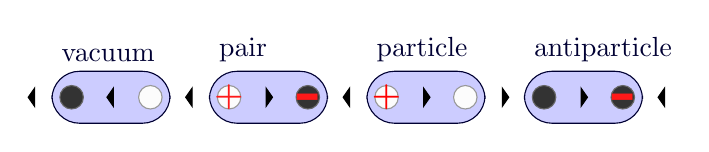
\begin{tikzpicture}[xscale = 1, yscale = 0.66]

            \draw[blue!20!black,fill=blue!20,rounded corners=10]
                (-0.25,0.5) node[above right] {vacuum} rectangle (1.25,-0.5);

            \draw[blue!20!black,fill=blue!20,rounded corners=10]
                (1.75, 0.5) node[above right] {pair} rectangle (3.25,- 0.5);

            \draw[blue!20!black,fill=blue!20,rounded corners=10]
                (3.75,0.5) node[above right] {particle} rectangle (5.25,-0.5);

            \draw[blue!20!black,fill=blue!20,rounded corners=10]
                (5.75, 0.5) node[above right] {antiparticle} rectangle (7.25,-0.5);
            
            \foreach \x in {0,3,6,7}
            \node [draw, circle, fill=white!20!black, minimum size=.1cm, scale=0.9, draw=white!40!black] at (\x,0) {};
        
            \foreach \x in {1,2,4,5}
            \node [draw, circle, fill=white!99!black, minimum size=.1cm, scale=0.9, draw=white!60!black] at (\x,0) {};
            
            \foreach \x in {0,1,2,4,8}
            \node[isosceles triangle, isosceles triangle apex angle=110,
                draw,fill=black, minimum size =0.03cm, inner sep=0.03cm, rotate=180] (T60) at (-0.5 + \x, 0){};
            
            \foreach \x in {3,5,6,7}
            \node[isosceles triangle, isosceles triangle apex angle=110,
                draw,fill=black, minimum size =0.03cm, inner sep=0.03cm] (T60) at (-0.5 + \x, 0){};
            \node[align=left, text=white!10!red,font=\large] at (1.998,0) {\textbf{+}};
            \node[align=left, text=white!10!red,font=\Huge] at (3.016,0) {\textbf{-}};
            \node[align=left, text=white!10!red,font=\Huge] at (7.016,0) {\textbf{-}};
            \node[align=left, text=red,font=\large] at (3.998,0) {\textbf{+}};
            \end{tikzpicture}}
        \end{figure}
        \pause
        \item Want periodic boundary conditions $\to$ net charge 0
        \pause
        \item Trotterization required temporal periodicity $\to$ same rule in the vertical direction
    \end{itemize}
\end{frame}



\begin{frame}[t]{$S = 1/2$ Cluster Algorithm}
    \begin{itemize}
        \setlength{\itemsep}{0.2cm}
        \item This translates to rules for clusters
        \item Use an ordering of the clusters according to their topology
        \vspace{-0.4cm}
    \begin{columns}
        \column{0.5\textwidth}
        \begin{figure}
            \centering
            \resizebox{\textwidth}{!}{
            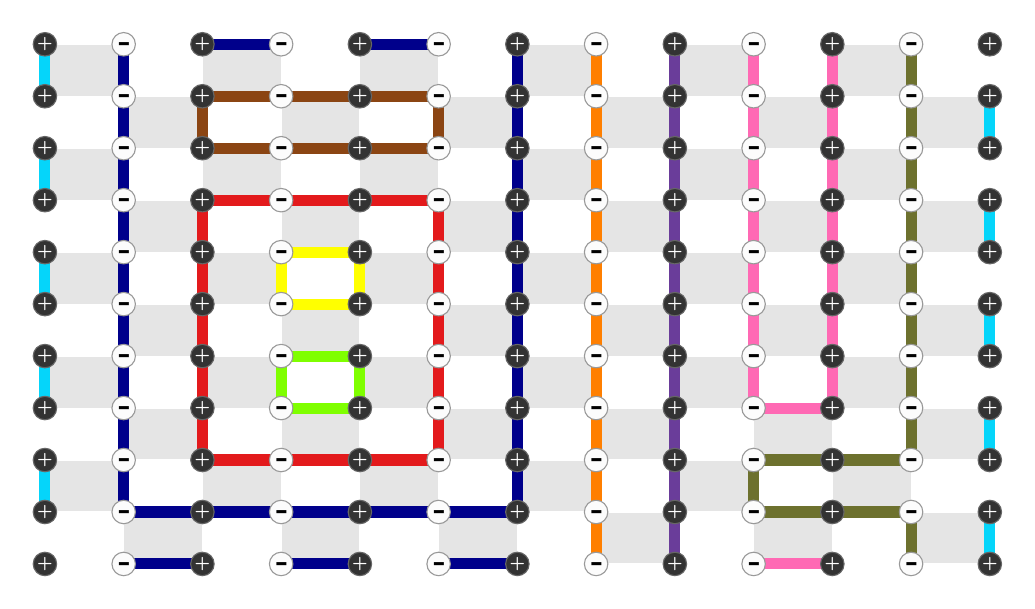
\begin{tikzpicture}[xscale = 1, yscale = 0.66]
                \foreach \x in {0,...,5}
                \foreach \y in {0,...,4}
                \filldraw[fill=black!10!white, draw=white] (2*\x,2*\y+1) rectangle (2*\x+1,2*\y+2);
                \foreach \x in {0,...,5}
                \foreach \y in {0,...,4}
                \filldraw[fill=black!10!white, draw=white] (2*\x+1,2*\y) rectangle (2*\x+2,2*\y+1);
            
           
                \draw[line width = 4, color1] (12,0) -- (12,1);
                \draw[line width = 4, color1] (0,1) -- (0,2);
                \draw[line width = 4, color1] (12,2) -- (12,3);
                \draw[line width = 4, color1] (0,3) -- (0,4);
                \draw[line width = 4, color1] (12,4) -- (12,5);
                \draw[line width = 4, color1] (0,5) -- (0,6);
                \draw[line width = 4, color1] (12,6) -- (12,7);
                \draw[line width = 4, color1] (0,7) -- (0,8);
                \draw[line width = 4, color1] (12,8) -- (12,9);
                \draw[line width = 4, color1] (0,9) -- (0,10);
        
        
                \draw[line width = 4, color2] (1,1) -- (1,10);
                \draw[line width = 4, color2] (1,0) -- (2,0);
                \draw[line width = 4, color2] (2,10) -- (3,10);
                \draw[line width = 4, color2] (3,0) -- (4,0);
                \draw[line width = 4, color2] (4,10) -- (5,10);
                \draw[line width = 4, color2] (5,0) -- (6,0);
                \draw[line width = 4, color2] (6,10) -- (6,1) -- (1,1);
        
        
                \draw[line width = 4, color3] (2,2) -- (5,2) -- (5,7) -- (2,7) -- (2,2);
        
                \draw[line width = 4, color4] (3,3) -- (4,3) -- (4,4) -- (3,4) -- (3,3);
        
                \draw[line width = 4, color5] (3,5) -- (4,5) -- (4,6) -- (3,6) -- (3,5);
        
                \draw[line width = 4, color6] (2,8) -- (2,9) -- (5,9) -- (5,8) -- (2,8);
        
                \draw[line width = 4, color7] (7,0) -- (7,10);
        
                \draw[line width = 4, color8] (8,0) -- (8,10);
        
                \draw[line width = 4, color9] (9,10) -- (9,3) -- (10,3) -- (10,10);
                \draw[line width = 4, color9] (9,0) -- (10,0);
        
                \draw[line width = 4, color10] (11,10) -- (11,2) -- (9,2) -- (9,1) -- (11,1) -- (11,0); 
        
                \foreach \x in {0,2,4,6,8,10,12}
                \foreach \y in {0,...,10}
                \node [draw, circle, fill=white!20!black, minimum size=.1cm, scale=0.9, draw=white!40!black] at (\x,\y) {};
            
                \foreach \x in {1,3,5,7,9,11}
                \foreach \y in {0,...,10}
                \node [draw, circle, fill=white!99!black, minimum size=.1cm, scale=0.9, draw=white!60!black] at (\x,\y) {};
            
                \foreach \x in {0,2,4,6,8,10,12}
                \foreach \y in {0,...,10}
                \node[align=left, text=white,font=\tiny] at (\x,\y) {\textbf{+}};
            
                \foreach \x in {1,3,5,7,9,11}
                \foreach \y in {0,...,10}
                \node[align=left, text=black,font=\large] at (\x + 0.016,\y) {\textbf{-}};

            \end{tikzpicture}
            }
        \end{figure}
        \column{0.5\textwidth}
        \begin{figure}
            \centering
            \resizebox{\textwidth}{!}{
            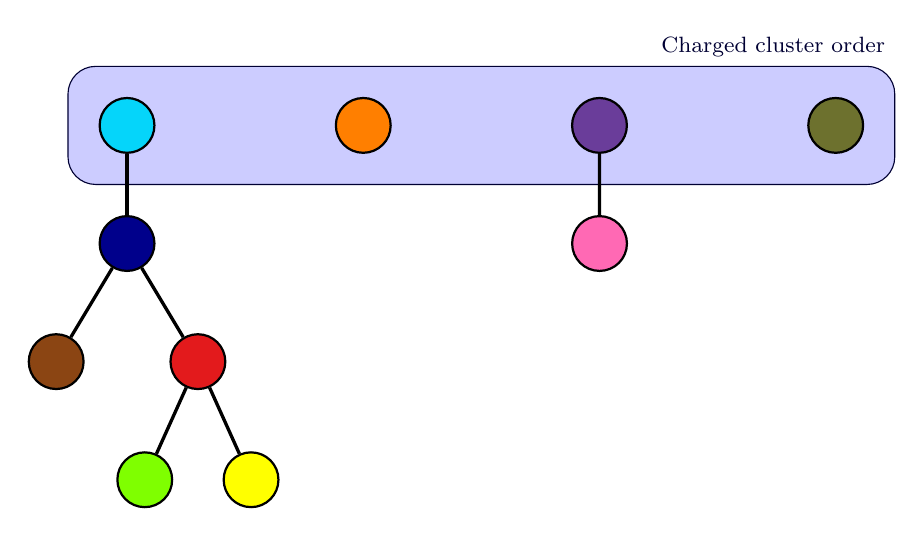
\begin{tikzpicture}[scale=1.5,font=\footnotesize]
            
                \draw[blue!20!black,fill=blue!20,rounded corners=10]
                (-0.5,-0.5) rectangle (6.5,0.5)
                node[above left] {Charged cluster order};
            
                \tikzset{
                % Two node styles for game trees: solid and hollow
                node1/.style={circle, draw, inner sep=7,fill=color1, thick},
                node2/.style={circle, draw, inner sep=7,fill=color2, thick},
                node3/.style={circle, draw, inner sep=7,fill=color3, thick},
                node4/.style={circle, draw, inner sep=7,fill=color4, thick},
                node5/.style={circle, draw, inner sep=7,fill=color5, thick},
                node6/.style={circle, draw, inner sep=7,fill=color6, thick},
                node7/.style={circle, draw, inner sep=7,fill=color7, thick},
                node8/.style={circle, draw, inner sep=7,fill=color8, thick},
                node9/.style={circle, draw, inner sep=7,fill=color9, thick},
                node10/.style={circle, draw, inner sep=7,fill=color10, thick}
                }
                
                % Specify spacing for each level of the tree
                
                \tikzstyle{level 1}=[level distance=10mm,sibling distance=25mm]
                
                \tikzstyle{level 2}=[level distance=10mm,sibling distance=12mm]
                    
                \tikzstyle{level 3}=[level distance=10mm,sibling distance=9mm]
            
                
                \node at (0,0)[node1]{}
                child[very thick]{node[node2]{}
                    child{node[node6]{}}
                    child{node[node3]{}
                        child{node[node4]{}}
                        child{node[node5]{}}
                    }
                };
            
                \node at (2,0)[node7]{};
            
                \node at (4,0)[node8]{}
                child[very thick]{node[node9]{}};
            
                \node at (6,0)[node10]{};
            \end{tikzpicture}}
            \end{figure}
    \end{columns}
    \pause
        \item Winding clusters are charged and must be flipped with alternating charge and net charge 0
        \item Non-winding clusters may only be flipped if their closest flipped ancestor is an odd number of levels higher in the tree
    \end{itemize}
\end{frame}

\begin{frame}[t]{$S = 1/2$ Cluster Algorithm}
    \begin{itemize}
        \setlength{\itemsep}{0.4cm}
        \item Need to generate all of these physical configurations with uniform probability
        \pause
        \item Count the number of legal physical configurations from the bottom up
        \pause
        \item Use weighted automaton to implement the rule for winding clusters:

    \begin{columns}
        \column{0.5\textwidth}
        \begin{figure}
            \centering
            \resizebox{0.6\columnwidth}{!}{
            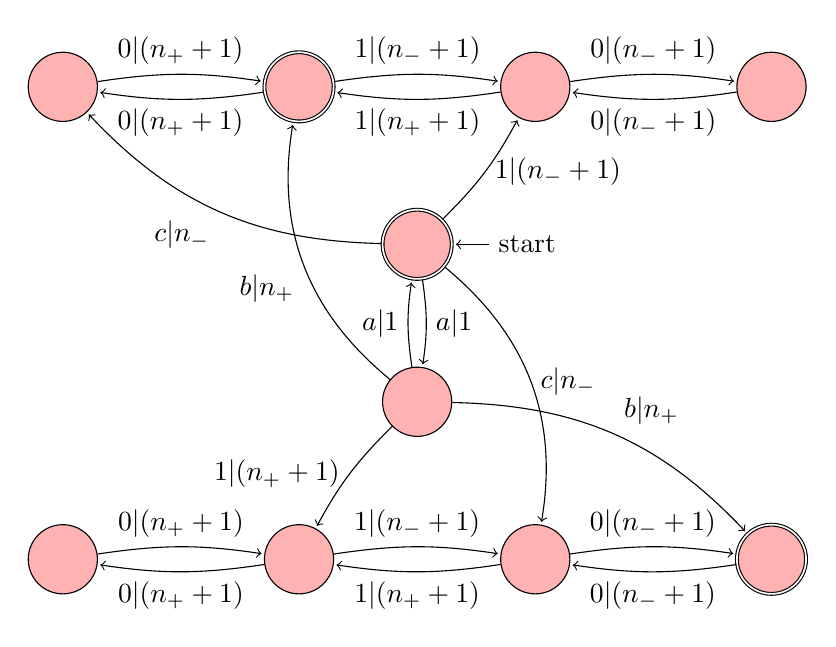
\begin{tikzpicture}[shorten >=1pt,node distance=2cm,on grid,auto] 
            \tikzstyle{every state}=[fill=red!30!white]
          
            \node[state, initial right, accepting] (q_5) at (4.5, 1) {};
            \node[state] (q_6) at (4.5, -1) {};
        
            \node[state] (q_1) at (0, 3) {};
            \node[state, accepting] (q_2) at (3, 3) {};
            \node[state] (q_3) at (6, 3) {};
            \node[state] (q_4) at (9, 3) {};
        
            \node[state] (q_7) at (0, -3) {};
            \node[state] (q_8) at (3, -3) {};
            \node[state] (q_9) at (6, -3) {};
            \node[state, accepting] (q_10) at (9, -3) {};
        
            \path[->]
            (q_1) edge [bend left=0.3cm] node {$0|(n_+ + 1)$}    (q_2)
            (q_2) edge [bend left=0.3cm]  node {$0|(n_+ + 1)$}   (q_1)
            (q_2) edge [bend left=0.3cm] node {$1|(n_- + 1)$}   (q_3)
            (q_3) edge [bend left=0.3cm] node {$1|(n_+ + 1)$}    (q_2)
            (q_3) edge [bend left=0.3cm] node {$0|(n_- + 1)$}    (q_4)
            (q_4) edge [bend left=0.3cm] node {$0|(n_- + 1)$}    (q_3)
            
            (q_5) edge [bend right=0.3cm] node [right] {$1|(n_- + 1)$}   (q_3)
            (q_5) edge [bend left=0.3cm] node {$a|1$}    (q_6)
            (q_6) edge [bend left=0.3cm] node {$a|1$}    (q_5)
            (q_6) edge [bend right=0.3cm] node [left] {$1|(n_+ + 1)$}    (q_8)
        
            (q_5) edge [bend left] node [right] {$c|n_-$}   (q_9)
            (q_6) edge [bend left] node {$b|n_+$}   (q_2)
            (q_5) edge [bend left=0.8cm] node {$c|n_-$}   (q_1)
            (q_6) edge [bend left=0.8cm] node {$b|n_+$}   (q_10)
        
        
        
            (q_7) edge [bend left=0.3cm] node {$0|(n_+ + 1)$}    (q_8)
            (q_8) edge [bend left=0.3cm]  node {$0|(n_+ + 1)$}   (q_7)
            (q_8) edge [bend left=0.3cm] node {$1|(n_- + 1)$}   (q_9)
            (q_9) edge [bend left=0.3cm] node {$1|(n_+ + 1)$}    (q_8)
            (q_9) edge [bend left=0.3cm] node {$0|(n_- + 1)$}    (q_10)
            (q_10) edge [bend left=0.3cm] node {$0|(n_- + 1)$}    (q_9);
        
          \end{tikzpicture}}
        \end{figure}
        \column{0.5\textwidth}
        \resizebox{\columnwidth}{!}{

          \begin{tabular}{| c | c |}
            \hline
            Symbol & Action  \\ \hline
            0 & Don't flip the charge, but flip the neutral clusters \\
            1 & Flip the charge and flip the neutral clusters \\
            a & Don't flip anything \\
            b & Flip the neutral clusters to a configuration with even parity\\
            c & Flip the neutral clusters to a configuration with odd parity \\ \hline
          \end{tabular}}
    \end{columns}
        \item The probability to flip each cluster can then be calculated
    \end{itemize}
\end{frame}

\section{Results}

\begin{frame}[t]{Comparison to exact diagonalization}
    \begin{itemize}
        \item Results for small lattices agree with exact diagonalization up to the Trotter error
    \end{itemize}
    \begin{figure}[t]
        \centering
        \begin{subfigure}{.5\textwidth}
          \centering
          \includegraphics[width=\linewidth]{Figures/comparison_lattice_width_16_beta_20.0.jpeg}
        \end{subfigure}%
        \begin{subfigure}{.5\textwidth}
          \centering
          \includegraphics[width=\linewidth]{Figures/difference_lattice_width_16_beta_20.0.jpeg}
        \end{subfigure}
    \end{figure}
    \begin{equation*}
        \mathcal{N}_{xy} = \left \langle \left(\hat{n}_x - \frac{1-(-1)^x}{2}\right) \left(\hat{n}_y - \frac{1-(-1)^y}{2}\right) (-1)^{(x+y)} \right \rangle = \langle \rho_x \rho_y \rangle
    \end{equation*}
\end{frame}

\begin{frame}[t]{Some nice results for the massless case}
    \begin{itemize}
        \item Algorithm can compute observables for large lattice sizes
    \end{itemize}
    \begin{figure}[t]
        \centering
        \begin{subfigure}{.5\textwidth}
          \centering
          \includegraphics[width=\linewidth,trim={0cm 0cm 0cm 0.8cm},clip]{Figures/susceptibility_lattice_width.jpeg}
        \end{subfigure}%
        \begin{subfigure}{.5\textwidth}
            \centering
            \includegraphics[width=\linewidth,trim={0cm 0cm 0cm 0.8cm},clip]{Figures/correlation_lattice_width_512.jpeg}
        \end{subfigure}
    \end{figure}
    \begin{equation*}
        \chi_\mathcal{E} = \sqrt{\frac{1}{(eN)^2} \left\langle \left(\sum_{n=0}^{N-1} \hat{E}_n\right)^2 \right \rangle}.
    \end{equation*}
\end{frame}

\begin{frame}[t]{Massive case}
    \begin{itemize}
        \setlength{\itemsep}{0.4cm}
        \item So far we had set $m = 0$
        \item One can reintroduce the mass
        \item The probability to flip each cluster becomes proportional to $e^{ -\epsilon \frac{m}{2} |C|}$ where $|C|$ is the size of the cluster
        \item This makes it harder to create many fermions
    \end{itemize}
\end{frame}

\begin{frame}[t]{Phase transition}
    \begin{itemize}
        \item The system exhibits a phase transition in the electric susceptibility at $m_c \sim 0.244$
        \vspace{-0.4cm}
        \begin{figure}[t]
            \centering
        \begin{subfigure}{.5\textwidth}
          \centering
          \includegraphics[width=\linewidth]{Figures/phase_transition.jpeg}
        \end{subfigure}%
        \begin{subfigure}{.5\textwidth}
            \centering
            \includegraphics[width=\linewidth]{Figures/critical_exponents.jpeg}
        \end{subfigure}
        \end{figure}
        \only<1>{
            \begin{equation*}
                \chi_\mathcal{E} = \sqrt{\frac{1}{(eN)^2} \left\langle \left(\sum_{n=0}^{N-1} \hat{E}_n\right)^2 \right \rangle }.
            \end{equation*}
        }
        \only<2>{
        \item Critical exponents $\nu \sim 1$, $\beta \sim 1/8$ from tensor network calculations\footcite{Rico2013} confirmed
        \vspace{0.3cm}
        }
    \end{itemize}
\end{frame}

\begin{frame}[t]{Critical slowing down}
    \begin{itemize}
        \setlength{\itemsep}{0.1cm}
        \item Large autocorrelation times around the phase transition
        \vspace{-0.4cm}
        \begin{figure}[t]
            \centering
            \begin{subfigure}{.5\textwidth}
            \centering
            \includegraphics[width=\linewidth]{Figures/autocorrelation_time.jpeg}
            \end{subfigure}%
            \begin{subfigure}{.5\textwidth}
                \centering
                \includegraphics[width=\linewidth]{Figures/critical_slowing.jpeg}
            \end{subfigure}
        \end{figure}
        \pause
        \item Scaling with at least $z \sim 2.5$ is comparatively bad
    \end{itemize}
\end{frame}

\section{Conclusion}

\begin{frame}[t]{Conclusion}
    \begin{itemize}
        \setlength{\itemsep}{0.5cm}
        \item Developed a cluster algorithm for the $S=1/2$ quantum link model
        \item Was able to reproduce known results
        \item It is the first cluster algorithm able to simulate quantum link models together with dynamical fermions (up to our knowledge)
    \end{itemize}
\end{frame}

\section{Outlook}

\begin{frame}[t]{Outlook}
    \begin{itemize}
        \setlength{\itemsep}{0.5cm}
        \item Can we improve the autocorrelation times?
        \pause
        \item Higher Spins are possible, the best algorithm I have constructed so far is $\mathcal{O}(V S^2)$
        \begin{itemize}
            \item Can study phase transition for higher spin, once implemented
        \end{itemize}
        \pause
        \item Wilson formulation ($S \to \infty$) configurations can be generated in $\mathcal{O}(V)$, but the reweight factors for the $E_n^2$ term diverge exponentially with the volume
        \begin{itemize}
            \item Can we find a better approach than reweighting?
        \end{itemize}
        \pause
        \item For 2+1 dimensions, physical fermion configurations can be generated, however, that does not fix the gauge field and a sign problem is introduced. 
        \begin{itemize}
            \item Can we solve this sign problem?
        \end{itemize}
    \end{itemize}
\end{frame}

\begin{frame}[allowframebreaks]{}
    \printbibliography
\end{frame}

\end{document}